We built and uses an Entity System as an underlying game engine framework.
The idea behind an entity system is that objects should be treated as pure aggregations of data containers, with game logic being separated from objects all together. Instead of having deep class hierarchies and chained method calls, logic for managing specific components is batched on all such components in the system. This provides some advantages over other approaches such that the architecture becomes more flexible and expendable. It is clearer how to add functionality and especially where. Another advantage from the batching is the scalability as it simplify parallel processing.

\subsection{Entity System}
An Entity System consists of three main parts: Entities, Components and Systems.
An Entity is simply a label or identifier of an object. A Component is a pure data containers, and each entity has a collection of none to several different components. A System consist of logic for working with a component type or a group of component types. How this differs from other traditional architectures can be seen in figure \ref{fig:SoftwareArchitectures}, which display a few standard game software architectures considering the aspects of structure regarding logic and data.
\begin{figure}[H]
  \centering
  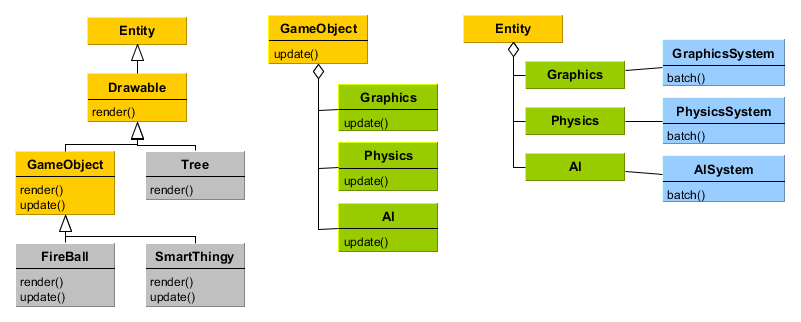
\includegraphics[width=\linewidth]{images/softwareArchitectures.png}
  \caption{A comparison of different game architectures. 
  To the left: A deep hierarchy architecture. 
  In the middle: A Component architecture or an Entity-Component System architecture. 
  To the right: An Entity System.}
  \label{fig:SoftwareArchitectures}
\end{figure}
The first architecture shown is a so called deep hierarchy architecture, a typical OOP architecture, in which inheritance is used to create more abstract objects from less abstract objects. In larger projects it easily lead to class explosion and blob class problems. The second architecture is one in which objects are created as aggregations of different components. Either there is one type for each object type, in which the components make up the entity but doesn't define it, or there is only one object (or entity) class and the components it is made up of defines it. The components all have individual communication needs and logic. The last architecture to the right is an Entity System, in which the data of the components is entirely separated from the logic. The logic is batched over all components of each type. Mick West (2007) writes about Entity-Component Systems. Boreal Games (2013) have an article on gemedev.net with a short but illustrative comparison between deep OOP architectures and Entity Systems. Alec McEachran (2013) explains in an interesting way, using for example linguistics, the benefits of using an Entity System compared to other traditional approaches. He writes about why it is generally so hard to keep the game structured and modular when using a deep OOP architecture and why Entity Systems improve code re-usage and promotes extendability and modularity. Adam Martin (2007) give a practical implementation of a Entity System and talks about its benefits in the light of MMORPGs. 	
\newpage
So, in an Entity System an object is an entity label and a collection of components that belong to it. The object is updated by different systems performing tasks on the components. An example used in this project is seen in figure \ref{fig:EntityComponentSystemExample}.
\begin{figure}[H]
  \centering
  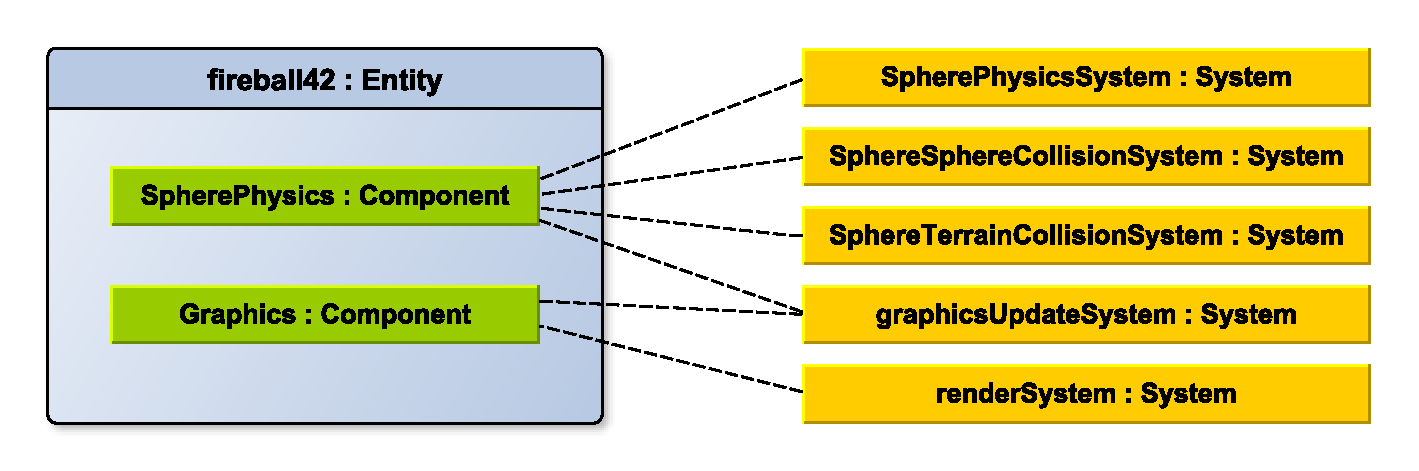
\includegraphics[width=0.9\linewidth]{images/EntityComponentSystemExample.eps}
  \caption{A lava stone (or fire ball) used in our demo. The renderSystem is in our current implementation not actually part of the Entity System, but it could easily be integrated. }
  \label{fig:EntityComponentSystemExample}
\end{figure}
Our Entity System is built using sophisticated meta template programming techniques. It is a compile time construct, enabling consistency verification, code generation and error correction. All components are controlled by the EntityManager class and each component type is stored continuous in memory. We provide an Entity class which work as an interface to the entity label and the components which builds up the component, this through the Entitymanager. The Entity interface is shown in figure 2.3 and an example of the construction of the fire ball in figure \ref{fig:EntityComponentSystemExample} is shown in figure 2.4. All access to components are reference based to minimize copying and the risk of pointer errors. Our system allows for components to require other components. This means that systems which work on multiple components can be proven to always work by fetching the component which require the others. The require check is performed at compile time and code is generated to handle the specific requirement-tree specified. The program writes part of itself to be maximum efficient and robustness, by specifications by the developer in the source code.
\begin{figure}[H]
  \centering
  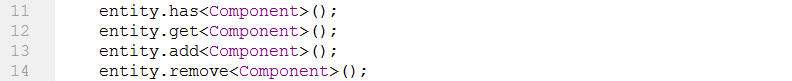
\includegraphics[width=0.9\linewidth]{images/entityInterfaceExample.png}
  \label{fig:EntityInterface}
  \caption{Entity Interface. Component is a place holder for any component type. \textit{has} return a boolean, \textit{get} return a reference to that component (if the entity consists of such a component), \textit{add} adds the component to the entity and returns a reference to it, \textit{remove} remove the component from the entity.}
\end{figure}
\begin{figure}[H]
  \centering
  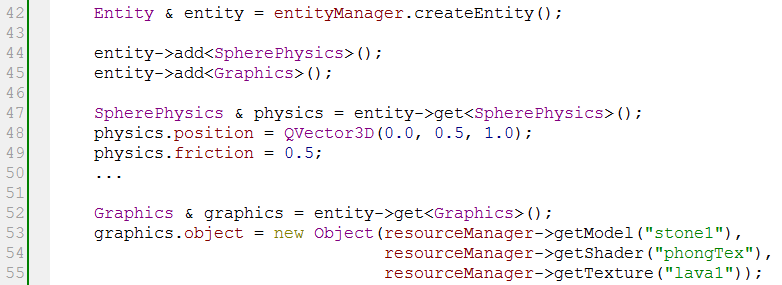
\includegraphics[width=0.9\linewidth]{images/entityCreationExample.png}
  \label{fig:EntitySetupExample}
  \caption{The creation and initiation of an entity.}
\end{figure}
A component is simply a \textit{struct} or a \textit{class} which inheritance the Component class. The only requirement is that it implements a getName() method returning the name of the component as a string. A simple example is shown in figure 2.5, and a more detailed component actually used is shown in figure \ref{fig:spherePhysics}.
\begin{figure}[H]
  \centering
  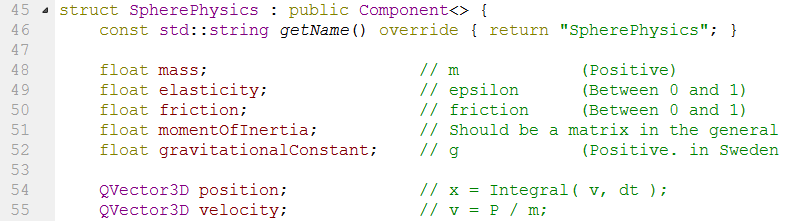
\includegraphics[width=0.9\linewidth]{images/SpherePhysicsPartExample.png}
  \label{fig:spherePhysicsPart}
  \caption{A part of the SpherePhysics component. The template argument \textit{$<>$} is empty, meaning that no system based on SpherePhysics require any other component to be present as well.}
\end{figure}
The component must be registered in the EntityManager before it is used. If it is used anywhere in the Entity System without registration a compile time error will be generated and supplied to the developer. Since C++11 didn't provide template parameter lists we have to use a define at this one place, until the next standard hopefully is released. The registration is shown in figure \ref{fig:entityInitializationExample}.
\begin{figure}[H]
\begin{subfigure}{\textwidth}
  \centering
  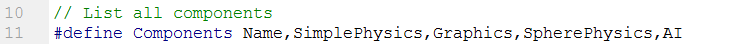
\includegraphics[width=0.9\linewidth]{images/componentList.png}
  \caption{}
  \label{fig:componentListExample}
\end{subfigure}%
\\
\begin{subfigure}{\textwidth}
  \centering
  
\includegraphics[width=0.9\linewidth]{images/entityManagerInstanciation.png}
  \caption{}
  \label{fig:entityManagerInstanciation}
\end{subfigure}
\caption[Ground textures]{\textit{Component registration. (a): Component is now an alias for the list of component types used in the Entity System. (b): The EntityManager is implemented with a list of every Component to be used in the Entity System.}}
\label{fig:entityInitializationExample}
\end{figure}
Systems are classes which must inheritance the System class and either overload \textit{processStep} (which is the action to be performed on a single component) or \textit{batch} if something involving multiple entities at the same time much be performed e.g. in the collision detection. An example of a simple dummy-system is shown in figure 2.7.
\begin{figure}[H]
  \centering
  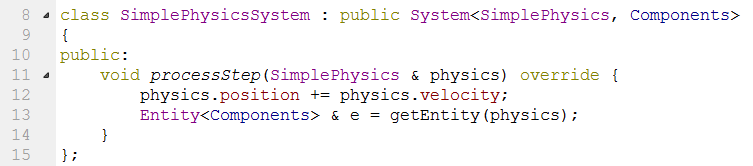
\includegraphics[width=0.9\linewidth]{images/simplePhysicsSystem.png}
  \label{fig:SimplePhysicsSystem}
  \caption{A dummy system. It iterates primarily over all SimplePhysics components. Illustrated is also the access to the entity from its component.}
\end{figure}
To guarantee consistency for systems requiring multiple component types, dependency between components is supported as shown in figure 2.5. Circular dependencies are supported as well. A system which require component A and B can then for example fetch all A, and if A require B then a B will be available to the system for each B since any Entity consisting of A will consist of B also. This is enforced by the Entity System such that when a component is added to an entity then any component required as well is also added, recursively. Similarly if a component is removed which other components belonging to the entity require. Then all components no longer supported are also removed, recursively. The code to check, add and remove components due to such requirements is generated by the Entity System such that no components are checked unnecessary for any component in any add/remove situation. This makes the system have the minimal overhead possible while still allowing arbitrary dependencies between components. 

The code generation is written using meta meta templates from our meta-library, also written for the project. An example of such a function call is shown in figure 2.8. What is shown is an except of the \textit{addComponent} method of the EntityManager, which is called by the Entity method \textit{add$<$Component$>$()} in turn. It generates all the \textit{has$<$Component$>$()} and \textit{add$<$Component$>$()} calls necessary to fulfill the requirement the current Component has and then calling all these methods. The \textit{add$<$Component$>$()} will in turn go through the same process, but with a possibly different component which requirements must be fulfilled, and so on until all requirements are fulfilled for all components in the dependency graph.
\begin{figure}[H]
\begin{subfigure}{\textwidth}
  \begin{lstlisting}
    // If additional Components are required, add these aswell (recursively)
      meta::FOR_EACH< typename Component::REQUIRED_COMPONENTS, // List (items) to iterate over
      
                      ADD_COMPONENT,                           // Template to apply
                                                               // on each item.
                      std::tuple<Component, Components...>,    // Additional template
                                                               // parameters to above template.
                      std::tuple<Entity<Components...>&>       // Argument types to the above
                                                               // templatet's execute-function.
                    >::execute(entity);
  
  \end{lstlisting}
  \label{fig:ADD_COMPONENT_FOREACH}
  \caption{}
\end{subfigure}%
\\
\begin{subfigure}{\textwidth}
  \begin{lstlisting}
    template<typename Element, typename Component, typename... Components>
    struct ADD_COMPONENT {
        static void execute(Entity<Components...> & e) {
            if(!e.template has<Element>()) {
                e.template add<Element>();
                Component c;
                Element el;
                std::cout << "Entity (" << e.getID() << ") warning: ";
                std::cout << "Adding \"" << c.getName() << "\" require \"" << el.getName()
                          << "\" which is missing, it is now automatically added.\n";
            }
        }
    };  
  \end{lstlisting}
  \label{fig:ADD_COMPONENT}
  \caption{}
\end{subfigure}
  \label{fig:codeCreationExample}
  \caption{Code generation of adding required components. (a): An except of the \textit{addComponent} method of the EntityManager, a meta meta template function call which assures that all components that are required, starting with the current Component is added to the entity. (b): The \textit{ADD\_COMPONENT} template used in (a). All lines except the first in the if-statement are there for debugging purposes.}
\end{figure}
The case of removing a component is slightly more advanced since it is a reverse problem of the problem outlined above: when a component is removed, any component requiring it must also be removed. It is solved in a concise fashion and implemented similarly to above, thanks to the powerful meta-library. See the source code for the actual implementation.

The benefits of our Entity Systems is that it is easy to use and is non-intrusive. It is easy to maintain, easy to extend, extremely efficient. It is trivial to parallelize calculations, e.g. divide the batching to be handled by different threads. Our system also verifies consistency at compile time. The later could probably be improved even more and open up vast possibilities of the construction of reliable software. Another advantage from the batching is the possibility of much higher performance, as we maximizing caching since components are continuous in memory, and minimizing cache misses since we minimize the need for conditional branches in many cases.

\newpage
\subsection{Rendering}
The rendering system is outside the entity system mainly because it is the largest individual part, and it was not known in the start of the project what information it needed exactly. So rather than potentially locking ourselves to an unusable architecture the renderer was placed beside the entity system rather than being integrated into it.

The rendering is done in two phases, the first calculates the shadows and second draws the world using the shadow information calculated in the first phase.

In order to correctly draw the growth some form of transparency was needed as the foilage used partly transparent textured polygons. As the textures where either completely transparent or completely opaque a simple alpha test was sufficient rather than sorting the trees. However the mipmaps calculated by OpenGL for the foilage where completely broken by the transparency, so these are disabled for the trees.

In order to be able to draw a sufficient number of trees and bushes a simple form of instancing is used. Each type of tree and bush exists in a separate list, that contains the model and texture for that particular object type and a position,orientation and scale for each instance in the list. The position,scale and orientaion is then used to compute a list of model matrices, that is uploaded to the shader as an array of uniforms.

The rocks on the other hand are drawn individually, using only a reference to a shared model objects, and individual matrices, as well as a specified shading program, indvidual rocks could be drawn using individual shaders if it was needed.

The water is always drawn last, as it is the only object in the world that is sempitransparent and thus the only object that needs to be sorted to be drawn properly. This does have the side effect of making the trees invisible from under the water tough. For future development a sorted render pass might be a good idea to implement, that would support arbitrary numbers of semitransparent objects, and draw them correctly relative to the trees/sorting-indepdent objects.

In general this demonstrates the need for a rendering pipeline that does not draw each object individually, but rather as a set of render passes, for example one for shadows, one for object geometry and one for post-processing.

Due to a rather lousy bush model with a great deal of z-fighting with itself, the depth mask is disabled while drawing bushes as this is considerably faster than finding or creating new models. It does require the bushes to be drawn last and that there are no other models needing this treatment, making it something of a hack.

\newpage
\subsection{Physics}
The physics used in this game is divided into three systems, all three processing all \textit{SpherePhysics} components in the Entity System. The physics is limited to 3D sphere physics as well as the interaction between spheres and a terrain mesh. In our current demo some of the physics is tuned to be less realistic but to allow for a greater chance of the lava balls to enter the ocean rather than get stuck at land. This is done in order to provide a better show for the audience. A major problem of the physics is that it is hard to dampen small oscillating motions of the rocks when they have come to an halt, or close to it. Decreasing the energy of the system was tried, which gives some results but makes the physics otherwise less spectacular as well as inhibit interesting backwards phenomenons.

\subsubsection{SpherePhysics}
SpherePhysics is a component dedicated to physics data, its content is seen in the code below in figure \ref{fig:spherePhysics}. The physics is capable of running backwards as well as forwards.
\begin{figure}[H]
\begin{lstlisting}
 struct SpherePhysics : public Component<> {
    const std::string getName() override { return "SpherePhysics"; }

    float mass;                     // m            (Positive)
    float elasticity;               // epsilon      (Between 0 and 1)
    float friction;                 // friction     (Between 0 and 1)
    float momentOfInertia;          // For a sphere: 6/12*m*radius^2
    float gravitationalConstant;    // g            (Positive. in Sweden at sea level: 9.82)

    QVector3D force;                // F = ... external events ...
    QVector3D linearMomentum;       // P = Integral( F, dt );
    QVector3D velocity;             // v = P / m;
    QVector3D position;             // x = Integral( v, dt );

    QVector3D torque;               // T = ... external events ...
    QVector3D angularMomentum;      // L = Integral( T, dt );
    QVector3D angularVelocity;      // w = L * Inverse(I)
    QQuaternion angularVelocity2;   // w = L * Inverse(I)
    QQuaternion rotation;           // r = Integral( w, dt );

    float radius;                   // Radius of the sphere
    QVector3D collisionVector;      // The sum of the vectors from all collisions

 };
\end{lstlisting}
\caption{The SpherePhysics component. All lava stones are composed by this component to enable physics and collision handling.}
\label{fig:spherePhysics}
\end{figure}

\subsubsection{SpherePhysicsSystem}
The sphere physics are based on the physics lab, with a generalization to 3D and using quaternions as the representation for rotation. The system require the current time step $dt$. which is used as the integration step in the Euler-forward integration used. This was sufficient for our needs, with no more advanced integration schemes necessary.\\
\\
The spheres are affected by external forces and torques, which then updates the rest of the physical states. At the end, any forces and torques has been handled and are set to zero, and finally the ever present gravitational force is added.

\subsubsection{SphereSphereCollisionSystem}
The sphere-sphere collision handling are based on the physics lab, with a generalization to 3D. The collision is handled by reversed impulse. Collisions give rise to torque, making he collisions seem very realistic.

\subsubsection{SphereTerrainCollisionSystem}
The sphere-sphere collision handling uses the terrains height and normal at the bottom of the sphere. It is otherwise similar to the SpherePshereCollisionSystem apart from that the terrain is considered to have infinite mass. A normal force is applied to the object to minimize noise from the gravity force. A friction force can be used if a more realistic collision is desirable. In our demonstration it isn't used since we had a limited amount of fire balls, so the fewer that got stuck on land the longer the volcano could spew out new fire balls.
